\documentclass[10pt]{article}

\usepackage{amsmath}
\usepackage{amsfonts}
\usepackage{amssymb}
\usepackage{gensymb}
\usepackage{fancyhdr}
\usepackage{textpos}
\usepackage{titlesec}
\usepackage[hyphens]{url}
\usepackage[hidelinks]{hyperref}
\usepackage{graphicx}
\graphicspath{ {./images/}}

\newtheorem{theorem}{Theorem}[subsection]
\newtheorem{lemma}[theorem]{Lemma}

\newcommand{\paren}[1]{\left ( #1 \right )}
\newcommand{\set}[1]{\left \{ #1 \right \}}
\newcommand{\floor}[1]{\left \lfloor #1 \right \rfloor}
\newcommand{\ceiling}[1]{\left\lceil #1 \right\rceil}
\newcommand{\cbrt}[1]{\sqrt[3]{#1}}
\newcommand{\dst}{\displaystyle}
\newcommand{\cycsum}{\sum_{\mathrm{cyc}}}
\newcommand{\symsum}{\sum_{\mathrm{sym}}}
\newcommand{\cycprod}{\prod_{\mathrm{cyc}}}
\newcommand{\symprod}{\prod_{\mathrm{sym}}}
\newcommand{\dang}{\measuredangle}
\newcommand{\ray}[1]{\overrightarrow{#1}} 
\newcommand{\seg}[1]{\overline{#1}}
\newcommand{\geoarc}[1]{\wideparen{#1}}
\DeclareMathOperator{\sign}{sgn}
\newcommand{\dg}{^\circ}
\newcommand{\reals}{\mathbb{R}}
\newcommand{\complexes}{\mathbb{C}}
\newcommand{\rationals}{\mathbb{Q}}
\newcommand{\integers}{\mathbb{Z}}
\newcommand{\naturals}{\mathbb{N}}
\newcommand{\field}{\mathbb{F}}

\DeclareMathOperator{\cis}{cis}
\DeclareMathOperator{\lcm}{lcm}

\newcommand{\themonth}{March}
\newcommand{\theyear}{2019}
\newcommand{\theissue}{The Big Document}
\newcommand{\thefirstday}{1}

\newcounter{day}
\setcounter{day}{\thefirstday}
\newcounter{solution}
\setcounter{solution}{1}
\newcounter{datenumber}
\setcounter{datenumber}{26} %starts on the 26th of March

\titleformat{\subsection}[runin]{\normalfont\large\bfseries}{\themonth~\arabic{datenumber}}{1em}{}

\renewcommand{\thesubsubsection}{Solution~\arabic{subsubsection}}

\setcounter{tocdepth}{2}

\pagestyle{fancy}
\fancyhf{}
\fancyhead[L]{\rightmark}
\fancyhead[R]{\theissue}
\cfoot{\thepage}

%Args: Problem # (optional), Source, Category, Statement
\newcommand{\problem}[4][0]{
	\newpage
	\subsection{[#3] \space #2} \hfill 
	{\large\textbf{Day \arabic{day}}} %| \arabic{subsection} \themonth~\theyear
	\begin{flushleft} #4 \end{flushleft}
	\vspace{1em}
	\addtocounter{day}{1}
	\addtocounter{datenumber}{1}
	\setcounter{solution}{1}
}

%Args: Problem # (optional), Sumbitter, UserID, Solution
\newcommand{\solution}[4][0]{
	\paragraph{Solution \arabic{solution}} \hfill submitted by #2 \hfill \texttt{#3}
	\begin{flushleft} #4 \end{flushleft}
	\addtocounter{solution}{1}
	\vspace{1em}
}

\begin{document}
	\begin{titlepage}
		\begin{textblock*}{2cm}(13.75cm,-4cm) \begin{flushright}\theissue \end{flushright} \end{textblock*}
		\vspace*{\stretch{1.0}}
		\begin{center}
			\LARGE\textbf{Mathematical Olympiads\\Discord Server}\\
			\vspace*{\stretch{3.0}}
			\Huge\textbf{POTD Solutions}\\
			\vspace*{\stretch{2.0}}
			\Large\textbf{\theissue}\\
			%\vspace*{\stretch{3.0}}
			%\large\textit{Compiled by server staff}\\
			\vspace*{\stretch{15.0}}
			\Large\textsc{Main Contributors}\\
			\vspace*{\stretch{0.7}}
			\normalsize{brainysmurfs, Daniel, Tony Wang (individual contributors listed next to each problem)}\\
			\vspace*{\stretch{0.7}}
			Discord Server Link: \url{https://discord.gg/m22vNrX}\\
			Problem Spreadsheet: \url{http://bit.ly/potd-history}\\
		\end{center}
		\vspace*{\stretch{2.0}}
	\end{titlepage}
\section{Introduction}

This document is an set of problems and solutions which have been listed in the \texttt{\#problem-of-the-day} channel of the Mathematical Olympiads Discord Server. Problems are selected from past contests and range from very easy to IMO3/6 level and beyond.

Although the document has been compiled by staff, solutions will be typically member-submitted. As these are problems ``of the day'', the set of problems is continually growing and thus solutions are welcome. If you wish to submit a solution, please send a direct message to the bot \texttt{Staff Mail} via the command \texttt{m.submit}. Alternatively, you may submit a pull request on Github. You will be credited if you wish.

The staff team are indebted to \texttt{www.imomath.org} for making available English translations of many national and international Mathematics Olympiads.

\paragraph{Tag system} Each problem is tagged according to its genre and difficulty. Genre is indicated using initials\footnote{\textbf{A}lgebra, \textbf{C}ombinatorics, \textbf{G}eometry, \textbf{N}umber theory and \textbf{C}ombinatorial \textbf{g}eometry.} and difficulty is indicated on a scale with 1 being very easy, 6 being the typical difficulty of an IMO1/4 problem, and 10 being the typical difficulty of an IMO3/6 problem. For example, a problem assigned the [NCg2] tag is an easy problem in number theory involving some combinatorial geometry.\\

Note that this document is a compilation of all the problems ever to be submitted. Monthly releases will also be available. 

\section{Problems}

These begin on the next page.

\problem[1]{2015 Romanian MoM, Q1}{N4}{Does there exist an infinite sequence of positive integers $a_1, a_2, a_3, \dots$ such that $a_m$ and $a_n$ are coprime if and only if $\lvert m - n \rvert = 1$?}

\solution[1]{SharkyKesa}{268970368524484609}{Suppose the primes are $p_1$, $p_2$, $p_3$, ... . Set $$a_1 = p_2 \cdot p_3$$and $$a_n = p_{n+2} \cdot p_{n-1} \cdot p_{n-3} \cdot p_{n-5} \cdots$$ Then it is trivial to show consecutive $a_i$ are co-prime, but the rest are not co-prime.\footnote{It would be great if someone were to provide a solution which explicitly showed how this sequence fulfilled the conditions of the problem.}}

\problem[2]{2018 IMO Shortlist, C1}{C5}{A rectangle $R$ with odd integer side lengths is divided into small rectangles with integer side lengths. Prove that there is at least one among the small rectangles whose distances from the four sides of $R$ are either all odd or all even.}

\solution[2]{SharkyKesa}{268970368524484609}{Colour in chessboard fashion with the corners as black, so the number of blacks is 1 greater than whites. Then there exists an internal rectangle with more blacks than whites, so it must have all corners as blacks, which means it satisfies the property that the distance to the sides is all odd or even.}

\problem[3]{2014 BMO2, Q2}{A4}{Prove that it is impossible to have a cuboid for which the volume, the surface area and the perimeter are numerically equal. (The perimeter of a cuboid is the sum of the lengths of all its twelve edges.)}

\solution[3]{Tony Wang}{541318134699786272}{Let the sides of the cuboid be $a$, $b$ and $c$. Furthermore let $X = abc$, $Y = 2(ab+bc+ca)$, and $Z=4(a+b+c)$. \\
Now suppose that $XZ = Y^2$, from $X=Y=Z$. Then this means that $$
4(a^2bc+b^2ca+c^2ab) = 4(a^2b^2+ab^2c+a^2bc+ab^2c+b^2c^2+abc^2+a^2bc+abc^2+a^2c^2)$$
So $$a^2b^2+ab^2c+b^2c^2+a^2bc+a^2c^2=0$$
Since $a$, $b$, $c > 0$ this is impossible, as required. 
}

\problem[4]{2015 APMO, Q4}{Cg4}{Let $n$ be a positive integer. Consider $2n$ distinct lines on the plane, no two of which are parallel. Of the $2n$ lines, $n$ are colored blue, the other $n$ are colored red. Let $\mathcal{B}$ be the set of all points on the plane that lie on at least one blue line, and $\mathcal{R}$ the set of all points on the plane that lie on at least one red line. Prove that there exists a circle that intersects $\mathcal{B}$ in exactly $2n-1$ points, and also intersects $\mathcal{R}$ in exactly $2n-1$ points.}

\solution[4]{SharkyKesa}{268970368524484609}{Consider the pair of red-blue lines with maximal angle between them, and consider a circle of increasing radius tangent to them through this angle. Trivial angle chasing yields that this circle must eventually intersect every other line (else you get a bigger angle)\footnote{Not rigorous yet. Additions are welcome.}}

\problem[5]{2005 IMO, Q4}{N5}{Determine all positive integers relatively prime to all the terms of the infinite sequence \[a_n=2^n+3^n+6^n -1,\, n\geq 1.\]}

\solution[5]{SharkyKesa}{268970368524484609}{Note that $2 \vert a_1=10$, $3 \vert a_2=48$. Now suppose $p > 3$ and p is prime. Then, 
\begin{equation}
$$\begin{align*}
a_{p-2} &= (3^{p-2} + 1)(2^{p-2} + 1) - 2\\
&= (1/3 + 1)(1/2 + 1) - 2\\
&= 4/3 \times 3/2 - 2 = 2 - 2\\
&= 0 \mod p
\end{align*}$$
\end{equation}
So $p \vert a_{p-2}$. Thus all primes $p$ eventually divide $a_n$, so only 1 satisfies.}

\solution[5]{SharkyKesa}{268970368524484609}{We proceed same as before for $p = 2, 3$. \\
Then, note that 
\begin{equation*}
$$
\begin{align*}
6a_{p-2} &= 6^{p-1} + 3 \times 2^{p-1} + 2 \times 3^{p-1} - 6\\
 &= 1 + 3 + 2 - 6\\
 &= 0 \mod p
\end{align*}$$
\end{equation*}
so we're done again}

\problem[6]{2007 Romanian Final MO, F9, Q3}{Cg3}{The plane is partitioned into unit-width parallel bands, each colored white or black. Show that one can always place an equilateral triangle of side length 100 in the plane such that its vertices lie on the same color.}

%reset date to April
\renewcommand{\themonth}{April}
\setcounter{datenumber}{1}

\problem[7]{2019 AFMO, Q3}{C0}{Suppose there are a line of prisoners, each of whom is wearing either a green or red hat. Any individual prisoner can see all the infinitely many prisoners and hats in front of them but none of the finitely many prisoners or hats behind them. They also can't see their own hat. In these circumstances, each prisoner then guesses the colour of their hat by writing it down, and the prison warden sets free any prisoner who correctly guesses the colour of their own hat. Assuming that the prisoners use the best strategy possible, what is the maximum guaranteed density of prisoners set free?}

\solution[7]{Tony Wang}{541318134699786272}{This problem was an April Fool's joke, with AFMO being an acronym for April Fool's Mathematical Olympiad. It would not appear on a mathematical competition for it's ``abuse of axiom of choice''. That being said, you can find a document explaining the question and solution here: \url{https://bit.ly/prisoner-problems-solution}.}

\problem[8]{2017 BMO1, Q3}{G2}{The triangle $ABC$ has $AB = CA$ and $BC$ is its longest side. The point $N$ is on the side $BC$ and $BN = AB$. The line perpendicular to $AB$ which passes through $N$ meets $AB$ at $M$. Prove that the line $MN$ divides both the area and the perimeter of triangle $ABC$ into equal parts.}

\problem[9]{2017 Canadian MO, Q2}{A5}{Define a function $f(n)$ from the positive integers to the positive integers such that $f(f(n))$ is the number of positive integer divisors of $n$. Prove that if $p$ is prime, then $f(p)$ is prime.}

\problem[10]{2015 IMO, Q1}{Cg6}{We say that a finite set $S$ of points in the plane is \textit{balanced} if, for any two different points $A$ and $B$ in $S$, there is a point $C$ in $S$ such that $AC = BC$. We say that $S$ is \emph{centre-free} if for any three different points $A, B$ and $C$ in $S$, there is no point $P$ in $S$ such that $PA = PB = PC$. \begin{enumerate} \item Show that for all integers $n \geq 3$, there exists a balanced set consisting of $n$ points.\item Determine all integers $n \geq 3$ for which there exists a balanced centre-free set consisting of $n$ points.\end{enumerate}}

\problem[11]{2015 IMO, Q2}{(FE)A9}{Let $\mathbb{R}$ be the set of real numbers. Determine all functions $f : \mathbb{R} \to \mathbb{R}$ such that, for all real numbers $x$ and $y$, \[f(f(x)f(y)) + f(x + y) = f(xy).\]}

\problem[12]{2013 BMO2, Q4}{NG5}{Suppose that $ABCD$ is a square and that $P$ is a point which is on the circle inscribed in the square. Determine whether or not it is possible that $PA$, $PB$, $PC$, $PD$ and $AB$ are all integers.}

\problem[13]{2018 EGMO, Q2}{N5}{Consider the set \[A = \left\{1 + \frac 1k : k = 1, 2, 3, \dots \right\}.\]	\begin{enumerate} \item Prove that every integer $x \geq 2$ can be written as the product of one or more elements of $A$, which are not necessarily different. \item For every integer $x \geq 2$, let $f(x)$ denote the minimum integer such that $x$ can be written as the product of $f(x)$ elements of $A$, which are not necessarily different. \end{enumerate} \noindent Prove that there exist infinitely many pairs $(x, y)$ of integers with $x \geq 2, y \geq 2$, and \[f(xy) < f(x) + f(y).\] \\ (Pairs $(x_1, y_1)$ and $(x_2, y_2)$ are different if $x_1 \neq x_2$ or $y_1 \neq y_2$.)}

\problem[14]{2017 NZ Squad Selection Test, Q5}{Cg4}{Let $A$ and $B$ be two distinct points in the plane. Find all points $C$ in the plane such that there does not exist a point $X$ in the plane with the property that $X$ is closer to both $A$ and $B$ than $C$.}

\problem[15]{2009 Russian MO (29th), Grade 11, Q1}{C2}{Some cities in a country are linked by roads, none of which intersect outside a city. Each city displays the shortest length of a trip (chain of roads) beginning in that city and passing through each of the other cities at least once. Prove that any two displayed lengths $a$ and $b$ satisfies $a \leq 1.5b$ and $b \leq 1.5a.$}

\problem[16]{2005 Korean MO (18th), Final Round, Q5}{N6-8}{Find all positive integers $m$ and $n$ such that both $3^m +1$ and $3^n +1$ are divisible by $mn$.}

\problem[17]{1999 Balkan MO (16th), Q1}{G4}{Let $D$ be the midpoint of the shorter arc $BC$ of the circumcircle of an acute-angled triangle $ABC$. The points symmetric to $D$ with respect to $BC$ and the circumcenter are denoted by $E$ and $F$, respectively. Let $K$ be the midpoint of $EA$. \begin{enumerate} \item[(a)] Prove that the circle passing through the midpoints of the sides of $\triangle ABC$ also passes through $K$. \item[(b)] The line through $K$ and the midpoint of $BC$ is perpendicular to $AF$. \end{enumerate}}

\problem[18]{2015/16 BMO1, Q6}{N5}{A positive integer is called \emph{charming} if it is equal to 2 or is of the form $3^i5^j$ where $i$ and $j$ are non-negative integers. Prove that every positive integer can be written as a sum of different charming integers.}

\problem[19]{2004 Swedish MO (44th), Final Round, Q3}{(FE)A3}{Find all functions $f$ satisfying $f(x)+x f(1-x) = x^2$ for all real $x$.}

\problem[20]{2018 IMO Shortlist, C2}{C5}{Let $n$ be a positive integer. Define a \emph{chameleon} to be any sequence of $3n$ letters, with exactly $n$ occurrences of each of the letters $a$, $b$, and $c$. Define a \emph{swap} to be the transposition of two adjacent letters in a chameleon. Prove that for any chameleon $X$, there exists a chameleon $Y$ such that $X$ cannot be changed to $Y$ using fewer than $3n^2/2$ swaps.}

\problem[21]{2009 Japanese MO, Final Round, Q2}{N3}{Let $N$ be a positive integer. Prove that if the sum of the elements in ${1,2,\dots,N}$ is even, then it is possible to paint each each element red or green so that the sum of the red numbers is equal to the sum of the green numbers.}

\problem[22]{2004 Swedish MO (44th), Final Round, Q4}{Cg6}{A square with integer side length $n \geq 3$ is divided into $n^2$ unit squares, and $n-1$ lines are drawn so that each square's interior is cut by at least one line. \begin{enumerate} \item[(a)] Give an example of such a configuration for some $n$. \item[(b)] Show that some two of the lines must meet inside the square \end{enumerate}}

\problem[23]{2018 Euclid Contest, Q10 (adapted)}{A5-A6}{In an infinite grid with two rows, each row continues to the left and right without bound. Each cell contains a positive real number. Prove that if each cell is the average of its three neighbours, then all the numbers in the grid are equal.}

\problem[24]{2015/16 BMO1, Q2}{G2}{Let $ABCD$ be a cyclic quadrilateral and let the lines $CD$ and $BA$ meet at $E$. The line through $D$ which is tangent to the circle $ADE$ meets the line $CB$ at $F$. Prove that the triangle $CDF$ is isosceles.}

\problem[25]{1993 IMO (34th), Q1}{(Poly)A5}{Let $n > 1$ be an integer and let $f(x) = x^n + 5x^{n-1} + 3$. Prove that there do not exist polynomials $g(x),h(x)$, each having integer coefficients and degree at least one, such that $f(x) = g(x)h(x)$.}

\problem[26]{2000 Dutch MO, Second Round, Q5 of 5}{C4}{Consider an infinite strip of unit squares numbered $1, 2, 3, \dots$. A pawn starting on one of these squares can, at each step, move between squares numbered $n$, $2n$, and $3n+1$. Show that the pawn will be able to reach the square $1$ after finitely many steps.}

\problem[27]{2005 Canadian MO (37th), Q2 of 5}{A4/N4}{Let ((a,b,c)) be a Pythagorean triple, i.e.\ a triplet of positive integers with ($a^2$ + $b^2$ = $c^2$). \begin{enumerate} \item[(a)] Prove that $(\left( \frac{c}{a} + \frac{b}{a} \right) ^2 > 8)$. \item[(b)] Prove that there are no integers $n$ and Pythagorean triples $(a,b,c)$ satisfying $\left( \frac{c}{a} + \frac{b}{a} \right) ^2 = n$. \end{enumerate}}

\problem[28]{2016 IMO (57th), Q1}{G6}{Triangle $BCF$ has a right angle at $B$. Let $A$ be the point on line $CF$ such that $FA=FB$ and $F$ lies between $A$ and $C$. Point $D$ is chosen so that $DA=DC$ and $AC$ is the bisector of $\angle{DAB}$. Point $E$ is chosen so that $EA=ED$ and $AD$ is the bisector of $\angle{EAC}$. Let $M$ be the midpoint of $CF$. Let $X$ be the point such that $AMXE$ is a parallelogram (where $AM \parallel EX$ and $AE \parallel MX$). Prove that $BD,FX$ and $ME$ are concurrent.}

\problem[29]{2018 Putnam, B3}{N3}{Find all positive integers $n < 10^{100}$ for which simultaneously $n$ divides $2^n, n - 1$ divides $2^n - 1$ and $n - 2$ divides $2^n - 2$.}

\problem[30]{2008 Polish MO, Second Round, Q4}{C4}{An integer is written in every square of an $n \times n$ board such that the sum of all the integers in the board is 0. A move consists of choosing a square and decreasing the number in it by the number of neighbouring squares (by side), while increasing the numbers in each of the neighbouring squares by 1. Determine if there is an $n \geq 2$ for which it is always possible to turn all the integers into zeros in finitely many moves.}

\solution[30]{Denial}{118831126239248397}{
Consider all the squares on the main diagonal of the board (shown in yellow and red), as shown in the figure below. Let $S$ represent the sum of all the numbers of the squares on the main diagonal. \\ 
\begin{center}
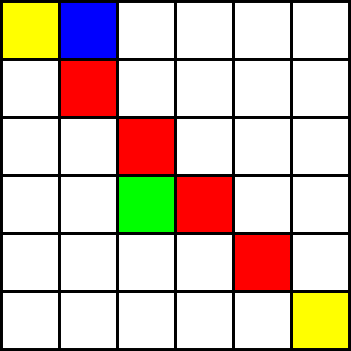
\includegraphics[scale=0.5]{q30-diagram}
\end{center}
\paragraph{Lemma 1: }$S$ is invariant mod 2. \\
Note that any 'move' performed will only affect the integers on the main diagonal if it is performed on either a square on the main diagonal (a yellow or red square in the diagram) or on a square adjacent to the main diagonal. We handle these cases separately. 
\begin{enumerate}
	\item[1. ]The move is performed on one of the squares of the main diagonal. Then if it is a yellow square, its number increases by $2$; whereas if it is a red square, its number increases by $4$. So $S$ will be invariant mod 2 in this case. Note that since squares on the main diagonal are not adjacent to each other, performing a move on one square will not affect any of the other squares. 
	\item[2. ]The move is performed on one of the squares adjacent to the main diagonal. Each of these squares is adjacent to exactly two squares on the main diagonal, and so the $S$ decreases by 2 and is thus invariant mod 2. 
\end{enumerate}
Note that having all 0's on the main diagonal means $S = 0 \mod 2$. However, since $S$ is invariant mod 2, then if the original configuration had $S = 1 \mod 2$, then it would be impossible to achieve the configuration with all the numbers being $0$. 
}

\problem[31]{2005 Serbia and Montenegro TST, Test 1, Q3}{A4}{Find all polynomials $P\left(x\right)$ that satisfy $P\left(x^2+1\right) = P\left(x\right)^2 + 1$ for all $x$.}

\problem[32]{2008 BMO2, Q3}{C5}{Adrian has drawn a circle in the $xy-$plane whose radius is a positive integer at most 2008. The origin lies somewhere inside the circle. You are allowed to ask him questions of the form "Is the point $(x,y)$ inside your circle?" After each question he will answer truthfully "yes" or "no". Show that it is always possible to deduce the radius of the circle after at most sixty questions. [Note: Any point which lies exactly on the circle may be considered to lie inside the circle.]}

\problem[33]{2013 IMO Shortlist, N3}{N6}{Prove that there exist infinitely many positive integers $n$ such that the largest prime divisor of $n^4 + n^2 + 1$ is equal to the largest prime divisor of $(n+1)^4 + (n+1)^2 + 1$.}

\problem[34]{2013 Australian TST, Q2}{G5}{Let $ABC$ be a triangle with orthocentre $H$. Let $D$ be the point such that $AHCD$ is a parallelogram. Let $M$ be the midpoint of $BC$, and the perpendicular from $M$ to $AB$ meet it at $E$. Let the line parallel to $BD$ through $A$ intersect $ME$ at $G$. Suppose $F$ is the midpoint of $ME.$ Show that $A, M, C$ and $F$ are concyclic if, and only if, $BF$ bisects $CG$.}

\problem[35]{2002 Taiwan MO (11th), Day 1, Q2}{N4/Cg4}{A lattice point $X$ in the plane is said to be \emph{visible} from the origin $O$ if the line segment $OX$ does not contain any other lattice points. Show that for any positive integer n, there is a square $ABCD$ of area $n^2$ such that none of the lattice points inside the square is visible from the origin.}

\problem[36]{1997 Balkan MO (14th), Q4}{(FE)A5}{Determine all functions $f:\mathbb{R}\to\mathbb{R}$ that satisfy $f(xf(x)+f(y))=(f(x))^2+y$ for all $x,y\in \mathbb{R}$.}

\end{document}
